\subsection{Power Apps}

Power Apps jest kolejnym składnikiem pakietu Office 365. Jest to środowisko Low-Code, dedykowane do tworzenia aplikacji biznesowych. Dzięki intuicyjnemu interfejsowi graficznemu, implementacja rozwiązań jest prosta, nawet dla osób bez zaawansowanej wiedzy programistycznej.

Power Apps jest zintegrowane z innymi usługami pakietu Office 365, takimi jak wcześniej opisane SharePoint czy Power Automate co znacznie rozszerza możliwości stworzonych aplikacji.

Rysunek \ref{fig:PowerAppsEditorOverview} przedstawia edytor programu. Zawiera on następujące elementy:
\begin{enumerate}
    \item \textbf{Pasek poleceń:} wyświetla inny zestaw poleceń w zależności od wybranego kontrolki.
    \item \textbf{Akcje aplikacji:} Opcje wyświetlania właściwości, dodawania komentarzy, sprawdzania błędów, udostępniania, podglądu, zapisu lub publikowania aplikacji.
    \item \textbf{Lista właściwości:} Lista właściwości wybranego obiektu.
    \item \textbf{Pasek formuł:} Tworzenie lub edycja formuły dla wybranej właściwości z użyciem jednej lub więcej funkcji.
    \item \textbf{Menu tworzenia aplikacji:} Panel wyboru umożliwiający przełączanie się między źródłami danych oraz wstawianie dodatkowych opcji.
    \item \textbf{Lista elementów aplikacji:} Pokazuje lementy obecne na ekranie w postaci drzewa.
    \item \textbf{Płótno/ekran:} Główne płótno do komponowania struktury aplikacji.
    \item \textbf{Panel właściwości:} Lista właściwości wybranego obiektu.
    \item \textbf{Ustawienia i wirtualny agent:} Ustawienia aplikacji lub uzyskanie pomocy od wirtualnego agenta.
    \item \textbf{Selektor ekranu:} Przełączanie się między różnymi ekranami w aplikacji.
    \item \textbf{Zmiana rozmiaru płótna:} Zmienianie rozmiaru wyświetlanego płótna podczas tworzenia aplikacji.
\end{enumerate}


\begin{figure}[h] % h - tu, t - góra, b - dół, p - strona dodatkowa
    \centering
    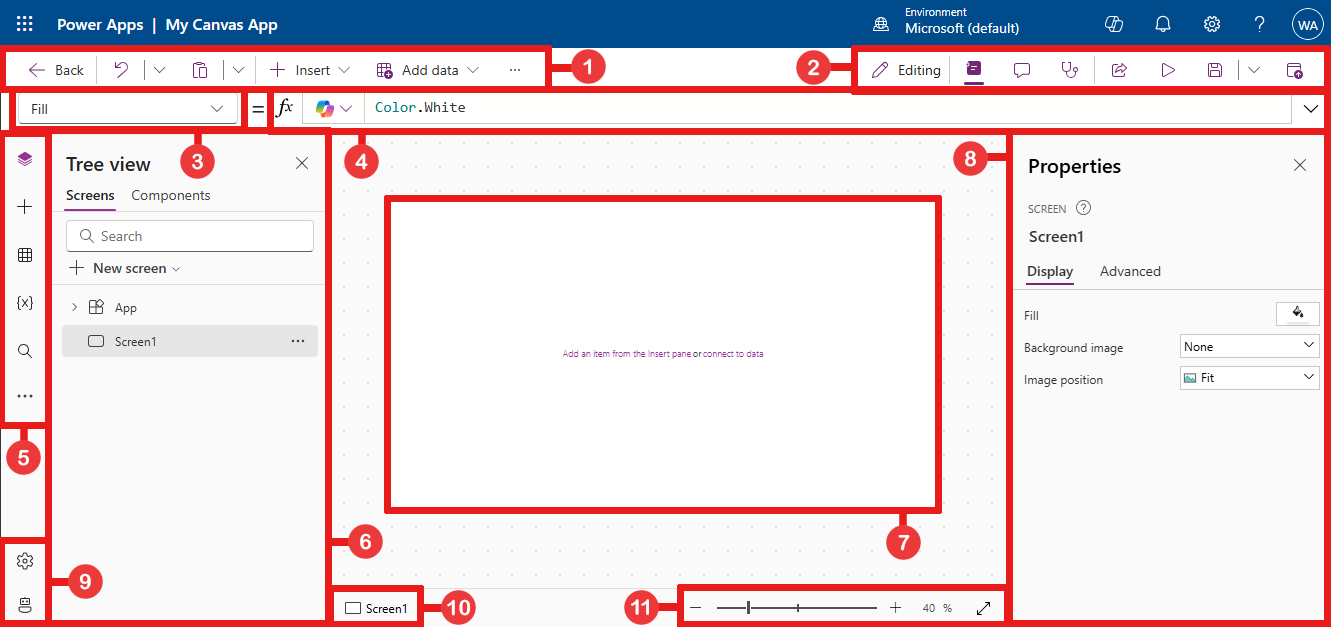
\includegraphics[width=\textwidth]{figures/PowerAppsOverview} 
    \caption{Edytor Power Apps} 
    \label{fig:PowerAppsEditorOverview}
\end{figure}
\textcolor{red}{LINK DO OBRAZKA I OPISU ELEMENTÓW: https://learn.microsoft.com/en-us/power-apps/maker/canvas-apps/power-apps-studio}

Dodawanie elementów do ekranów aplikacji odbywa się poprzez przeciąganie ich z biblioteki i upuszczanie w wybranym miejscu. Każdy komponent, może zostać skonfigurowany według potrzeb użytkownika poprzez edycje \emph{właściwości}. Możemy określić między innymi wypełnienie czy pozycję \emph{X} i \emph{Y} na ekranie, ale niektóre obiekty mają też unikalne właściwości takie jak \emph{OnSelect} \footnote{OnSelect -- określa akcje, które zostaną wykonane po naciścięciu elementu} dla przycisku.

Power Apps pozwala na stworzenie spersonalizowanej aplikacji dostosowanej do motywu organizacji a przy połączeniu z innymi serwisami, utworzone rozwiązania mogą być bardzo zaawansowane minimializując przy tym czas potrzebny na ich implementacje.
\vspace{15cm}

Ekrany aplikacji, komponowane za pomocą tego rozwiązania, porównywalne są z tymi, które można stworzyć w standardowych środowiskach programistycznych (jak np. JavaScript czy .NET), jednak proces ich tworzenia jest prostszy, ze względu na obecność edytora wizualnego. Umożliwia on korzystanie z gotowych komponentów w aplikacji, takich jak przyciski, pola danych wejściowych, listy, tabele, grafiki etc.




Power Apps jest kolejnym składnikiem pakietu Office 365. które umożliwia tworzenie aplikacji w środowisku Low-Code. Zostało zaprojektowane tak, aby było intuicyjne w obsłudze, pozwalając na projektowanie interaktywnych aplikacji, nawet przez użytkowników bez zaawansowanej wiedzy programistycznej.

Power Apps integruje się z innymi usługami i narzędziami z pakietu Microsoft 365, takimi jak SharePoint czy Power Automate, dzięki czemu znajduje wszechstronne zastosowania i pozwala na tworzenie uniwersalnych aplikacji usprawniających pracę.

Interfejsy użytkownika aplikacji, komponowane za pomocą tego rozwiązania, porównywalne są z tymi, które można stworzyć w standardowych środowiskach programistycznych (jak np. JavaScript czy .NET), jednak proces ich tworzenia jest prostszy, ze względu na obecność edytora wizualnego. Umożliwia on korzystanie z gotowych komponentów w aplikacji, takich jak przyciski, pola danych wejściowych, listy, tabele, grafiki etc.


